\documentclass{article}
\usepackage{amsfonts, amsmath, amsthm, hyperref}
\usepackage{mathrsfs, color}
\usepackage{comment}
\usepackage{enumitem}
\usepackage{graphicx}
\usepackage{caption}
\usepackage{subcaption}
\usepackage{matlab-prettifier}

\newtheorem{theorem}{Theorem}[section]
\newtheorem{corollary}[theorem]{Corollary}
\newtheorem{proposition}[theorem]{Proposition}
\newtheorem{lemma}[theorem]{Lemma}
\newtheorem{definition}[theorem]{Definition}
\newtheorem{question}[theorem]{Question}
\newtheorem{remark}[theorem]{Remark}
\newtheorem{example}[theorem]{Example}
\newtheorem{open-problem}[theorem]{Open Problem}

\def\mike#1{\noindent
\textcolor{green}
{\textsc{(Mike:}
\textsf{#1})}}

\def\jon#1{\noindent
\textcolor{blue}
{\textsc{(Jon:}
\textsf{#1})}}

\def\kemon#1{\noindent
\textcolor{red}
{\textsc{(Kemon:}
\textsf{#1})}}

\title{Math 5900 Final Paper}
\author{Jon Facinelli and Kemon Lardas}
\date{\today}

\graphicspath{{images/}}

\begin{document}

\maketitle

\section{Introduction}
There are countless states to the Rubik’s Cube puzzle, that is unless you count the 43,252,003,274,489,856,000 possible positions on your standard $3\times 3$ cube.  These states are created from the 54 visible squares (9 on each side) and 26 “cubies” all along a central axis.  There are corner cubies, edge cubies, and center cubies: corners have 3 faces exposed, edges have 2 faces exposed, and the center has one face exposed.  The goal of a Rubik’s Cube is to complete a series of turns in order to get the same color on each individual side: these colors are usually represented by white, red, blue, green, orange, and yellow.  What originally caught our eye about solving a Rubik’s Cube is the concept of God’s number, the maximum minimum number of moves required to solve a cube from any state.  God’s number for a $3 \times 3$ cube is 20; this means that out of the approximate 43 quintillion possible positions, the maximum number of moves that it would take to get to the solved state from any arbitrary state would be 20.  Now you can imagine the computer power necessary to go through every permutation, so our goal is to go through a process that simplifies God’s number using linear algebra. When you consider subgames you change what a move is, making the definition context dependent, but part of this process includes listing out all the possible moves for the sake of our research.  To represent these moves, we ended up adopting the Singmaster notation which describes the faces/turns in terms of the user looking at the front face, F:
\begin{itemize}
    \item U: turns the up face 90 degrees clockwise
    \item D: turns the down face 90 degrees clockwise
    \item L: turns the left face 90 degrees clockwise
    \item R: turns the right face 90 degrees clockwise
    \item F: turns the front face 90 degrees clockwise
    \item B: turns the back face 90 degrees clockwise
    \item U': turns the up face 90 degrees counterclockwise
    \item D': turns the down face 90 degrees counterclockwise
    \item L': turns the left face 90 degrees counterclockwise
    \item R': turns the right face 90 degrees counterclockwise
    \item F': turns the front face 90 degrees counterclockwise
    \item B': turns the back face 90 degrees counterclockwise
    \item $U^2$: turns the up face 90 degrees counterclockwise
    \item $D^2$: turns the down face 180 degrees 
    \item $L^2$: turns the left face 180 degrees 
    \item $R^2$: turns the right face 180 degrees 
    \item $F^2$: turns the front face 180 degrees
    \item $B^2$: turns the back face 180 degrees
\end{itemize}

Throughout this paper we will be thinking of the cube in a fixed position defined by the faces represented above.  We will not be rotating the cube in space, so for example the F move is always well-defined.

Other experts who have researched the Rubik’s Cube and the linear algebra behind it have also found this notation to be useful.  Janet Chen showed in \text{\cite{chenGroupTheory}} how the arrangement of a Rubik’s Cube can be represented by four categories:
\begin{itemize}
    \item The positions of the corner cubies, represented by $\sigma \in S_8$
    \item The positions of the edge cubies, represented by $\tau \in S_{12}$
    \item The orientation of the corner cubies, represented by $x \in (\mathbb{Z}/3\mathbb{Z})^8$
    \item The orientation of the edge cubies $y \in (\mathbb{Z}/2\mathbb{Z})^{12}$
\end{itemize}
Each piece of data plays a distinct part in what state the cube is in.  Thus she decides to represent it as a four-tuple ($\sigma, \tau, x, y$).  This is a valid standpoint because a corner cubie will have the same colors on each of its 3 exposed sides no matter where it is positioned on the cube.  The same can be said about the 2 exposed sides of an edge cubie, and only 1 exposed side of a center cubie.  Our research does not follow this exact path in creating this tuple, but the way it is viewed is similar when looking at the Rubik’s Cube as a group.

\subsection{The Rubik's Cube Group}
The Rubik's cube, based off of how it is arranged, can be described as a permutation group called the \emph{Rubik's Cube Group}, which we will refer to as $\mathcal{R}$.  By numbering the cube as represented by \textit{Figure 1} we are able to make a 54-tuple that tracks the positions of each of the cubies. Then solved state, which we label $\sigma_0$, would look as follows: 
$$\sigma_0 = \begin{pmatrix}
                1 & 2 & 3 & ... & 54\\
                1 & 2 & 3 & ... & 54
             \end{pmatrix}$$
\begin{figure}[ht]
    \centering
    \begin{subfigure}[b]{0.5\textwidth}
        \centering
        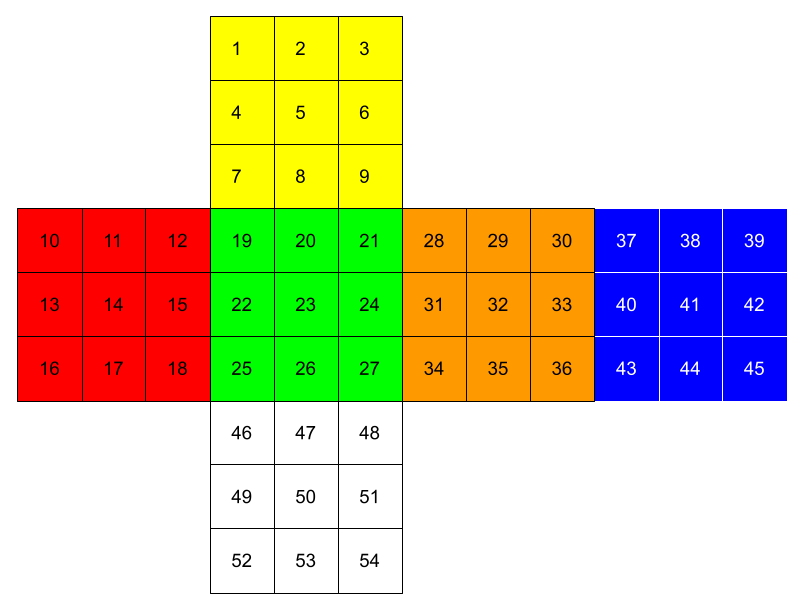
\includegraphics[scale=0.2]{images/Cube_Numbering.png}
        \caption{Solved Permutation}
        \label{fig:solved permutation}
    \end{subfigure}
    \hfill
    \begin{subfigure}[b]{0.5\textwidth}
        \centering
        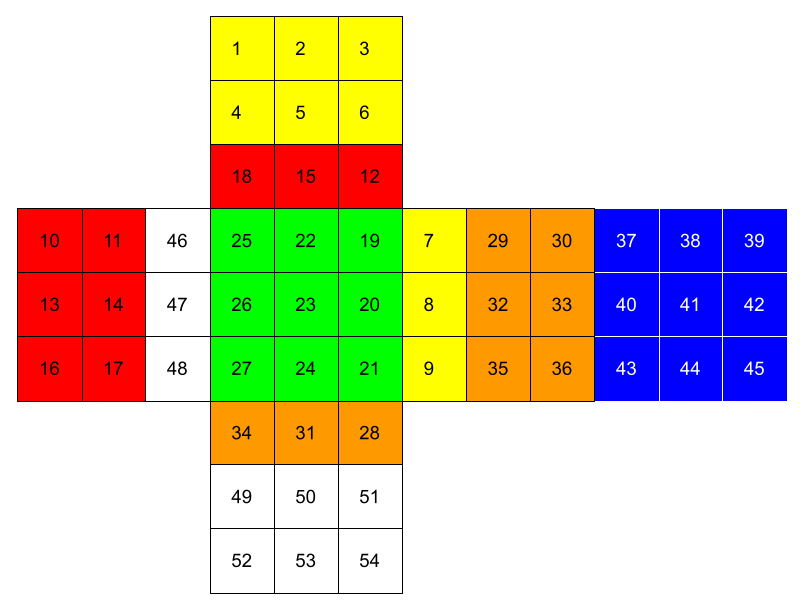
\includegraphics[scale=0.2]{images/Cube_Numbering_Front.png}
        \caption{$\sigma_F$}
        \label{fig:clockwise front turn}
    \end{subfigure}
    \caption{Permutation Examples}
    \label{fig:three graphs}
\end{figure}
For each of the face turns described earlier we can track the changes of the 54-tuple.  In \textit{Figure 1 (b)} we can see turning the front face the 54-tuple can be represented by 5 disjoint 4 cycles: $(20\ 24\ 26\ 22), (18\ 7\ 28\ 48), (31\ 47\ 15\ 8), (12\ 9\ 34\ 46), (19\ 21\ 27\ 25)$ which we will refer to as, $\sigma_F$.  Following this process we can generate disjoint cycles for the other 5 moves, they are as follows:
\begin{itemize}
    \item $\sigma_B = (1\ 16\ 54\ 30), (2\ 13\ 53\ 33), (3\ 10\ 52\ 36), (38\ 42\ 44\ 40), (37\ 39\ 45\ 43)$
    \item $\sigma_U = (1\ 3\ 9\ 7), (2\ 6\ 8\ 4), (10\ 37\ 28\ 19), (11\ 38\ 29\ 20), (12\ 39\ 30\ 21)$
    \item $\sigma_D = (16\ 25\ 34\ 43), (17\ 26\ 35\ 44), (18\ 27\ 36\ 45), (47\ 51\ 53\ 49), (46\ 48\ 54\ 51)$
    \item $\sigma_R = (3\ 43\ 48\ 21), (6\ 40\ 51\ 24), (9\ 37\ 54\ 27), (28\ 30\ 36\ 34), (29\ 33\ 35\ 31)$
    \item $\sigma_L = (1\ 19\ 46\ 45), (4\ 22\ 49\ 42), (7\ 25\ 52\ 39), (10\ 12\ 18\ 16), (11\ 15\ 17\ 13)$
\end{itemize}
These 6 permutations can be combined to represent other permutations on the cube as well, for example $\sigma_F\sigma_F$ is the permutation representation of Singmaster's $F^2$ in \text{\cite{Singmaster1981}}.  As we will be counting these double moves as their own move we will shorthand this notation to $\sigma_F^2$.  It is important to note that the ordering of moves in Singmaster's notation is opposite of what we will using for the computations of our permutations.  So, the Singmaster moves $UF$, which normally represent a clockwise turn of the ``up'' face followed by a clockwise turn of the ``front'' face, for our purposes will be represented by $\sigma_F \sigma_U$.

With these 6 permutations, we can use them to generate what we will be calling the Rubik's Cube group, $$\mathcal{R} = 
\langle \sigma_F, \sigma_B, \sigma_U, \sigma_D, \sigma_R, \sigma_L \rangle.$$  
As $\mathcal{R}$ is a subset of permutations on a 54-tuple, it is clear that $\mathcal{R} < S_{54}$.  This next paragraph covers various definitions from abstract algebra, for all definitions see \cite{doi:https://doi.org/10.1002/0471469882.ch3}.  This group inherits closure from $S_{54}$.  This group must also have an identity, in this case that will be our solved state, $\sigma_0$, or what will be known as the ``empty move''. It is worth noting that the group inherits associativity from $S_{54}$ as well.  An example of associativity would be performing $\sigma_U (\sigma_F \sigma_D)$, this permutation results in the same permutation as $(\sigma_U \sigma_F) \sigma_D$.  The only change is the grouping of the moves not the order in which they are done to the cube.  Based on the counterclockwise Singmaster notation described earlier, we can use this to determine the inverse of a permutation.  We can create a counterclockwise 90 degree rotation of the front face by reversing each of the 5 cycles of $\sigma_F$, which yields us: $\sigma_F^{-1} = (20\ 22\ 26\ 24), (18\ 48\ 28\ 7), (31\ 8\ 15\ 47), (12\ 46\ 34\ 9), (19\ 25\ 27\ 21)$.  By following a similar process we obtain inverses for the other cycles.  Using these inverse moves we can show that any inverse of a permutation is the inverse moves of a permutation in reverse order.  For example, we can arbitrarily select a set of moves, $\sigma_{M_1}\ \sigma_{M_2}\ \sigma_{M_3}$, the inverse of this permutation would be $\sigma_{M_3}^{-1}\ \sigma_{M_2}^{-1}\ \sigma_{M_1}^{-1}$.

It is important to understand that by restricting which moves are used as generators, we can create different subgroups of $\mathcal{R}$.  A great example of this is the group generated by only 180 degree turns of the faces.  By only using these double moves, we create what can be thought of as a ``sub-game" of the original puzzle with only being able to reach a smaller number of permutations.  These ``sub-games" are distinct from the original game.  We also note that all relevant questions about the original game can also be asked about these ``sub-games".  An example of one of these ``sub-games" is the group generated by $\langle \sigma_U^2,\ \sigma_D^2,\ \sigma_F^2,\ \sigma_B^2,\ \sigma_R^2,\ \sigma_L^2 \rangle < \mathcal{R}$.  There are various other subgroups that can be made by move restrictions.  Due to the smaller order of these subgroups, we will be exploring God's number of the double moves, as well as others, in more detail later.

\subsection{Cayley Graph}
For our purposes, we wanted to represent the Rubik's Cube Group, $\mathcal{R}$, as a graph in order to determine more about the Rubik's cube as a whole.  The best way to represent a group as a graph is using a Cayley graph, first implemented by Arthur Cayley in 1878 \cite{godsil01}.  Cayley graphs are meant to represent finite graphs and as such often are used to visualize groups.  A Cayley graph, $\Gamma$ is defined by a group, $G$, and a generating set, $S$, and are written as $\Gamma(G, S)$.  Thus we can define that: $$u \sim v \iff u,v \in G \text{ and } u-v \in S.$$  

Following the definition for a Cayley graph shown above, one of the graphs we are studying is, $$\Gamma(\mathcal{R},\langle \sigma_F, \sigma_F^{-1}, \sigma_B,\sigma_B^{-1}, \sigma_U, \sigma_U^{-1}, \sigma_D, \sigma_D^{-1}, \sigma_R, \sigma_R^{-1}, \sigma_L, \sigma_L^{-1} \rangle),$$ which is defined as:
$$\sigma \sim \tau \iff \sigma,\tau \in \mathcal{R} \text{ and}$$ $$ \sigma\tau^{-1} \in \langle \sigma_F, \sigma_F^{-1}, \sigma_B,\sigma_B^{-1}, \sigma_U, \sigma_U^{-1}, \sigma_D, \sigma_D^{-1}, \sigma_R, \sigma_R^{-1}, \sigma_L, \sigma_L^{-1} \rangle.$$  Using different subgroups and/or subsets as described earlier we are able to create various different graphs of sub-games of the Rubik's cube as well.  These graphs will be defined later when we define the research that we have done.

Structuring our group specifically as a Cayley graph is important because of the property of vertex transitivity.  Naively speaking a graph is vertex transitive if every vertex behaves the same as every other vertex, in other words, the vertex cannot be determined based solely on its surrounding edges.  More formally, a graph, $\Gamma$, is vertex transitive if for all $v_1,v_2 \in V(G)$ there exists an automorphism $f$ such that $f(v_1) = v_2$. For all relevant graph theory definitions see: \cite{godsil01}.
\begin{theorem}
    Every Cayley graph $G(X,S)$ is vertex transitive
\end{theorem}
\begin{proof}
    Fix $x_1, x_2 \in V(G)$.  Let $f: X \to X$ be a function such that $f(x) = x + x_2 - x_1$. \\
    Thus we show: $f(x_1) = x_1 + x_2 - x_1 = x_2$.\\
    As G is a Cayley graph it is clear that, $x \sim y \iff x-y \in S$.\\
    Using this we can show that $f(x) \sim f(y) \in G $ if $f(x) - f(y) \in S$. \\
    
    We compute, $f(x) - f(y) = x + x_2 -x_1 - (y +x_2-x_1) = x - y \in S.$ \\
    Therefore $f$ is an automorphism.
\end{proof}
This is crucial to understanding how a random walk on the graph relates to the Rubik's cube.  For this case as our graph is vertex transitive that means that a random walk from one vertex has the same properties as from any other vertex.

In addition to vertex transitivity, the diameter of a graph is also important to give attention to since it can be used to relate to God's Number.  Simply put, when we define the diameter it is the shortest longest path between all pairs of vertices in a graph.  When we are looking at a Rubik's Cube, God's Number is identical to this description as it is the shortest longest path to get from any arbitrary state to the solved state.

\begin{proposition}
Let $G_S$ be an arbitrary set of moves $\{\sigma_1, \sigma_2, ... , \sigma_n\}$ that describes a sub-game of the Rubik's cube.  Then, $diam(\Gamma(\mathcal{R}, G_S))$ = God's number for the sub-game of $G_S$.
\end{proposition}
For our paper we will be treating God's number as the diameter of a Cayley graph and they will be used interchangeably.

\subsection{Adjacency and Normalized Laplacian Matrix}
Using our graph of the cube, we are able to create an adjacency matrix that will be able to further our understanding of the Rubik's cube.  An \emph{adjacency matrix} is a matrix with its rows and columns labeled by the vertices of the graph which simply tells you whether or not two vertices are adjacent to each other.  This matrix is filled strictly with 1s and 0s, where a 1 represents two vertices that are adjacent to each other (an edge) and a 0 represents the latter.  The notation for this is the following: $$A_{ij} = \begin{cases} 1 &  i \sim j \\ 0 & i \not\sim j \end{cases},$$ where i and j represent the vertex of each row and column, and eigenvalues represented by $\lambda_1 \geq \cdots \geq \lambda_n$.  When talking about the diagonal of an adjacency matrix, it must be filled with zeros because a vertex can not be adjacent to itself.  With this information, the Cayley Graph is given more purpose and the Rubik’s Cube Group begins to seem more clear when represented this way.

The Laplacian Matrix, L, can be defined as a matrix measuring to what extent a graph differs at one vertex from its values at nearby vertices.  It is expressed as the degree matrix subtracted by the adjacency matrix: $$L = D - A$$  Using this matrix we are able to derive the \textbf{Normalized Laplacian Matrix} which can be defined by $$\mathcal{L} = D^{-1/2}(D-A)D^{-1/2}$$ The eigenvalues, $0 = \mu_1\leq \cdots \leq \mu_n$, found from this matrix will help us to extract Kemeny's Constant for certain subgroups of $\mathcal{R}$ talked about later in this paper.

\begin{theorem}
If a graph G is d-regular then $\lambda_1,\cdots, \lambda_n$ are eigenvalues of A $\iff$ the eigenvalues of $\mathcal{L}$ are $\mu_n = 1 - \frac{\lambda_n}{d}$. 
\end{theorem}

\begin{proof}
    Let G be regular and the eigenvalues of the Adjacency Matrix be $(\lambda_1,\cdots, \lambda_n)$ and the eigenvalues of the Normalized Laplacian Matrix be $(\mu_1,\cdots, \mu_n)$
    
    $\mathcal{L} = D^{-1/2}(D-A)D^{-1/2} = I - D^{-1/2}AD^{-1/2} = I - D^{-1}A = I - \frac{1}{d}A$\\
    Therefore, $\mathcal{L}$ is similar to $I - D^{-1}A$.\\
    Thus, $\mu$ is an eigenvalue of $\mathcal{L}$ if $1 - \mu$ is an eigenvalue of $D^{-1}A$.\\
    Which means, $\mathcal{L} = I - \frac{1}{d}A$ gives us the eigenvalues of the Normalized Laplacian in terms of the Adjacency Matrix, $\mu_n = 1 - \frac{\lambda_n}{d}$.\\  Thus, $(\lambda_1,\cdots, \lambda_n)$ are eigenvalues of A and $\mu_n = 1 - \frac{\lambda_n}{d}$ are eigenvalues of $\mathcal{L}$. 

\end{proof}

A \emph{walk} of length t in a graph is an ordered sequence $(v_1,v_2,v_3,...,v_i,v_{i+1})$ such that $v_i \sim v_{i+1}$.  In our case we can take any random walk on a given Cayley Graph in order to find how many moves it would take on average to get from one state to the next, or "the length of the walk".  For example, in a Cayley Graph representing a Rubik's cube subgroup, if $(v_1,v_3,v_4,v_7)$ is the shortest possible walk to get from $v_1$ to $v_7$ then there is a set of moves that is done to show $v_1 \sim v_3, v_3 \sim v_4,$ and $v_4 \sim v_7$ within this walk.  It is here where Kemeny's Constant becomes of interest to us.  \emph{Kemeny's constant} \text{\cite{breen2022kemenys}} is the expected length of a random walk on any given graph.  We are able to get this value \text{\cite{breen2022kemenys}} by taking the sum of the inverse of the eigenvalues of the Normalized Laplacian Matrix: $$\sum^{n}_{i=2}\frac{1}{\mu_i}$$  By finding this matrix along with its eigenvalues, $\mu$, we are able to find the length of the average walk on any subgroup of the Rubik's Cube Group represented by a Cayley Graph.

\begin{lemma}
$(A^k)_{ij}$ = the number of k-walks from $v_i$ to $v_j$
\end{lemma}

\begin{theorem}
$q(A) - 1 \geq \mathrm{diam}(G)$\text{\cite{ahmadi2013minimum}}
\end{theorem}

\begin{proof}
    Let $(\lambda_1,\cdots, \lambda_n)$ be the eigenvalues of an adjacency matrix $A$. \\
    We can construct the characteristic polynomial $f(x) = det(A - xI)$. Thus, $\lambda_i$ is an eigenvalue of A $\iff f(\lambda_i) = 0$. \\
    Since A is a symmetric matrix, we can rewrite this as $f(A) = \prod(x - \lambda_i)$.\\
    Using this characteristic polynomial we can create a minimal polynomial, which is the smallest nonzero polynomial that satisfies matrix $A$, such that $g(A) = 0$.  For our case, as A is symmetric, $g(x)$ is the polynomial with each distinct eigenvalue as a linear factor.\\
    We can show: $$0 = g(A) = \prod^t_{i=1}(A-\lambda_i) = \sum^t_{i=0} c_iA^i.$$
    From here we want to show that the given matrices $I, A, A^2, ..., A^d$ are linearly independent.  We define that $d$ is the diameter of the graph of $A$ and the vertices $v_1,...,v_d$ are on a shortest path from $v_1$ to $v_d$, which exists by the definition of diameter.\\
    Lets assume that $$c_0I + c_1A + ... + c_{d-1}A^{d-1}+ c_dA^d = [\Vec{0}].$$
    By Lemma 1.4, we know that matrices $A, ..., A^d$ are populated with the amount of walks of length $k$ from vertex $i$ to vertex $j$, and we will be ordering the first $d$ columns to be the vertices on a shortest path of length $d$. \\
    We will only focus on the first row of each matrix which then defines the amount of walks of length $k$ for vertex $1$. \\
    As the the distance from $v_1$ to $v_d$ is of length $d$ we will see that the value for the $d^{th}$ column for matrices $I, ..., A^{d-1}$ is 0. \\
    Thus, as $A^d$ is the only matrix that has a nonzero value in the $d^{th}$ column. \\
    By our original statement we then see that for the first row, $$c_0(0) + c_1(0) + ... + c_{d-1}(0)+ c_d(\text{some positive value}) = [\Vec{0}],$$$$\text{which leads us to show that }c_d = 0.$$
    Following this pattern we see that as $c_d = 0$, $A^{d-1}$ becomes the only matrix with a nonzero value in the $(d-1)^{th}$ column, which makes $c_{d-1} = 0$.\\
    This pattern continues across all of the matrices until finally we see that $$c_0 = c_1 = ... = c_{d-1} = c_d = 0.$$
    By our lemma we have now shown that the shortest walk from $i$ to $j$ is of length $d$. Then, as the minimal polynomial is a nontrivial linear combination of $I, A, ..., A^t$ which sums to $0$. This means that $I,A, ..., A^t$ are linearly dependent. Since the first $d$ powers are linearly independent, we know we must have $t>d$. 
\end{proof}


\section{Our Methodology}
In this section we are going to discuss our process on determining God's number.  We will be using the subgroup $\mathcal{DS} = \langle\sigma_F^2\sigma_B^2,\sigma_U^2\sigma_D^2,\sigma_L^2\sigma_R^2\rangle$, as the example to show this process, however we will be showing our findings for other subgroups in less detail later.

\subsection{Maple}
While going through the process of trying to determine God’s Number, we wanted to try and create a group that could represent the entire Rubik’s Cube.  Lucky enough Maple already had a pre-built one shown above, namely "RubiksCubeGroup".  This group returns a permutation group using the 6 generators we have talked about previously in this paper: front, back, left, right, up, and down.  To confirm whether or not this group was legitimate we were able to use a command shown in our code that returned the order of the entire RubiksCubeGroup, and this gave us exactly what we expected at approximately 43 quintillion.

\begin{figure}[ht]
    \centering
        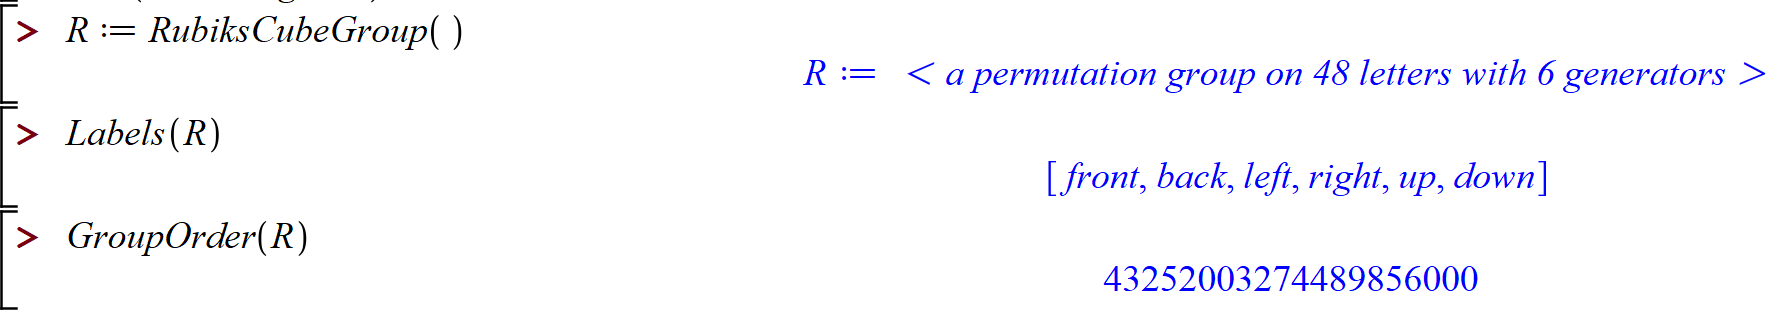
\includegraphics[scale=0.6]{images/MapleRC.png}
        \caption{Rubiks Cube Group in Maple}
\end{figure}

\begin{figure}[ht]
    \centering
        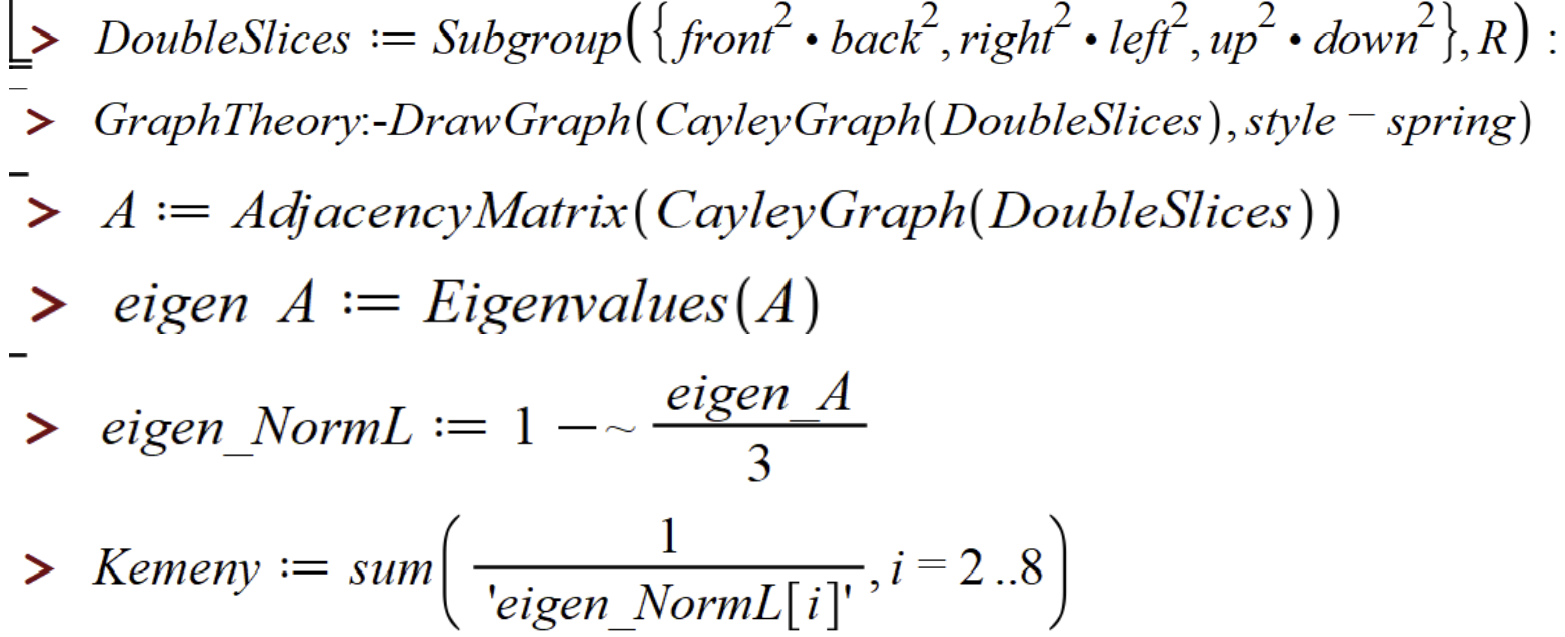
\includegraphics[scale=0.6]{images/MapleCode.png}
        \caption{Maple Code for Double Slice Moves}
\end{figure}

Now that we knew the pre-built group that Maple gave us was legit, we decided to make a simple subgroup that would allow us to look at God’s number on a simpler scale.  After some trial and error of going through subgroups that were too large for Maple to handle, we landed on one that was small and easy to comprehend consisting of three generators, double slice moves (shown in Figure 3 above).  Since the group order for double slices was relatively small at 8, we figured that it would be easy for us to compose a Cayley Graph shown below.  

\begin{figure}[ht]
    \centering
        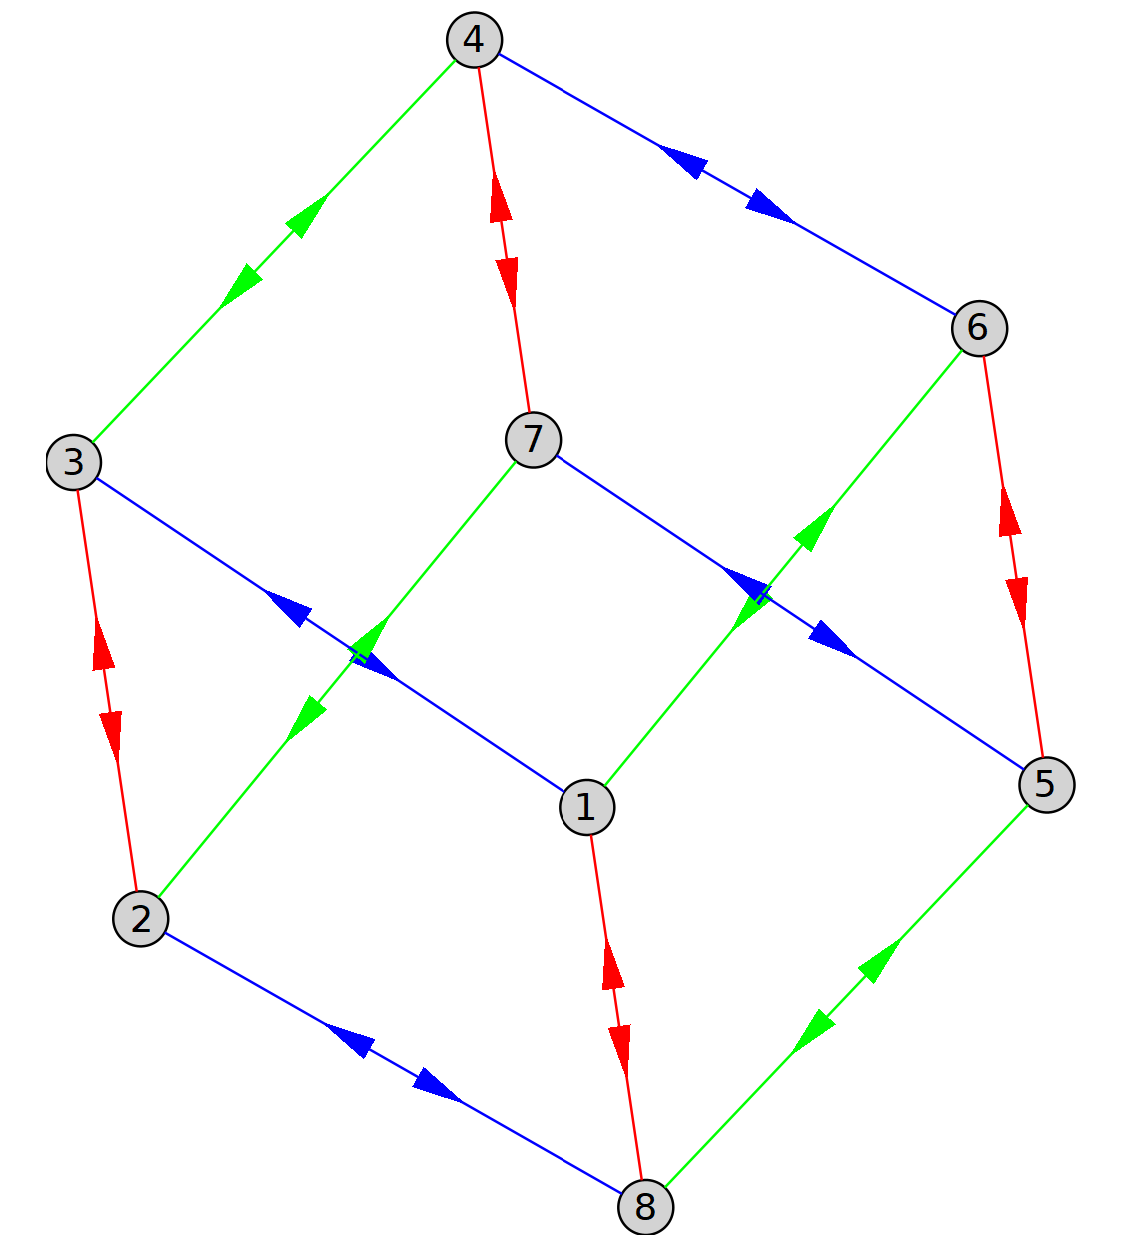
\includegraphics[scale=0.6]{images/CayleyGraph.png}
        \caption{Cayley Graph $\Gamma(\mathcal{R},\mathcal{DS})$}
\end{figure}

In this figure the color of each edge represents a generator move from the $\mathcal{DS}$ subgroup.  For the sake of this example lets say blue represents $\sigma_F^2 * \sigma_B^2$, red represents $\sigma_R^2 * \sigma_L^2$, and green represents $\sigma_U^2 * \sigma_D^2$.  Each of these edges on the graph symbolize how to get from one arbitrary state to the next strictly using double slices.  So if we wanted to get from vertex 3, $v_3$, to vertex 1, $v_1$, all we would have to do is $\sigma_{F}^2 * \sigma_{B}^2$.  If we wanted to move between two of the furthest arbitrary states on the graph (let's say $v_3$ to $v_5$), we would do $\sigma_F^2 * \sigma_B^2$, then $\sigma_R^2 * \sigma_L^2$, and finally $\sigma_U^2 * \sigma_D^2$.  However, since this graph is 3-regular (meaning that every vertex contains 3 edges) we can rearrange those moves in any order and still get from $v_3$ to $v_5$; that being said, $\sigma_R^2 * \sigma_L^2$, then $\sigma_F^2 * \sigma_B^2$, and finally $\sigma_U^2 * \sigma_D^2$ would also be a successful set of moves.  

After generating the Cayley Graph we were able to produce the Adjacency Matrix of the same subgroup, $\mathcal{DS}$, shown in Figure 5 below.  The first row represents $v_1$ and the other vertices that it is adjacent to, so there is a 1 in the third, sixth, and eighth column of this row because $v_1$ is adjacent to $v_3$, $v_6$, and $v_8$.  The same reasoning can be used for rows 2-8 as they each respectively represent $v_2$ through $v_8$.  The diagonal of the matrix is filled with zeros because no vertex can be adjacent to itself.   

\begin{figure}[ht]
    \centering
        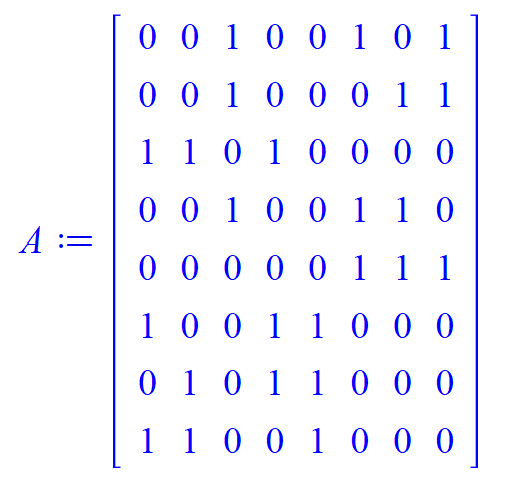
\includegraphics[scale=0.9]{images/AdjancencyMatrix.png}
        \caption{Adjacency Matrix (A)}
\end{figure}

Given the Adjacency Matrix, we were able to retrieve the eigenvalues, $(\lambda_1,\cdots,\lambda_8)$, shown in Figure 4 below.  The significance behind $(\lambda_1,\cdots,\lambda_8)$ is they are able to give us the eigenvalues of the Normalized Laplacian Matrix, $(\mu_1,\cdots,\mu_8)$ using the formula $$\mu_i = 1-\frac{\lambda_i}{\text{degree of matrix}}.$$  Thus in our code we computed $1-\frac{(\lambda_1,\cdots,\lambda_8)}{3}$, which spit out $(\mu_1,\cdots,\mu_8)$ shown below.  Therefore, using the formula for Kemeny's Constant in Section 1.4, we get a value of $\frac{29}{4}$ or $7.25$.  This represents the expected length of a random walk on $\Gamma(\mathcal{R},\mathcal{DS})$.  

\begin{figure}[!ht]
    \centering
    \begin{subfigure}[b]{0.4\textwidth}
        \centering
        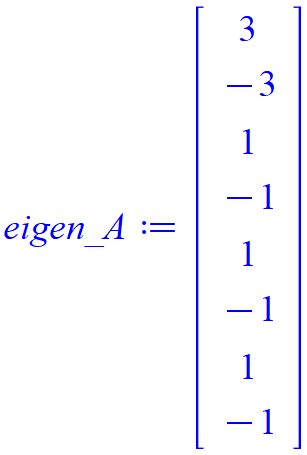
\includegraphics[width=0.5\textwidth]{images/AdjEigen.png}
        \caption{Eigenvalues $(\lambda_1,\cdots,\lambda_8)$}
        \label{fig:Adjacency eigenvalues}
    \end{subfigure}
    \hfill
    \begin{subfigure}[b]{0.4\textwidth}
        \centering
        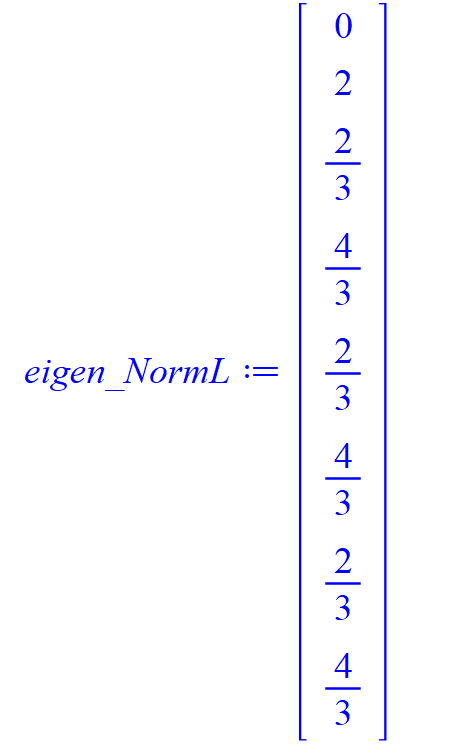
\includegraphics[width=0.5\textwidth]{images/NormEigen.png}
        \caption{Eigenvalues $(\mu_1,\cdots,\mu_8)$}
        \label{fig:Normalized eigenvalues}
    \end{subfigure}
    \caption{Adjacency and Normalized Eigenvalues}
    \label{fig:two sets}
\end{figure}

After finishing the whole process of creating a subgroup all the way down to finding Kemeny's Constant, we grew more curious to see what other subgroups we could find using Maple.  We wanted to take on more sizeable subgroups to try and see if we could replicate what we did for double slice moves, but on a larger scale.  The first signs of success in a larger subgroup was the generating set of double face turns, when we were able to have Maple compute an Adjacency Matrix with a group order of 2,592.  Although this seemed promising, we failed when trying to compute the eigenvalues of this matrix.  This is where we began to look for a better solution outside of Maple.

\subsection{Matlab}
After falling short on generating eigenvalues in Maple, we chose to shift our work to Matlab as it is more geared toward the final steps of our work.  Ultimately we ended up using Matlab not only to calculate the eigenvalues of the adjacency matrices we were creating but also to normalize the eigenvalues, solve for Kemeny's constant, and determine the distinct number of eigenvalues the matrix had.

Converting our previous work to Matlab was simpler than we had originally thought.  Maple does a great job in allowing matrices to be converted to many different file types including ones specific to Matlab.  We chose to work with a csv file as it was easier for us to process in Matlab, thus our code for importing the data is tailored to a csv file.  When replicating this project any type of matrix file should work however our code would need to be adjusted based on the file type. It is worth noting that the way the matrix is formatted in the csv file is dependent on the size of the matrix.  If a matrix is too big the csv file instead of displaying the matrix itself, lists in each row, the row, the column and non-zero value of the matrix in that order.  Due to our adjacency matrix being symmetric and only having ones as non-zero entries we were able to simplify the code for generating a larger sized matrix.  Shown below is the csv command in maple, as well as the Matlab code for formatting both smaller and larger formatted files.
\begin{figure}[ht]
    \centering
        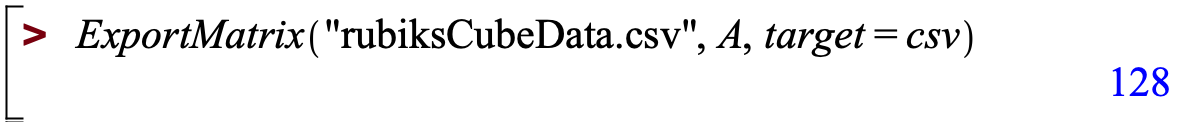
\includegraphics[scale=0.6]{images/ExportingMatrix.png}
        \caption{Maple code for exporting matrix}
\end{figure}
\begin{lstlisting}[
frame=single,
numbers=left,
style=Matlab-Pyglike]
% Matrix maker for smaller formatted matrices

% Reads in the data from a provided path of csv file 
path = 'data/rubiksCubeData.csv'; % Adjust to file path/name
data = readmatrix(path);

% Instanciates a matrix of all zeros
n = 8; % Adjust to input size of adjacency matrix
M = zeros(n, n);

% Populates the matrix based on the data
for row = 1:n
    for col = 1:n
        M(row, col) = data(row, col);
    end
end
\end{lstlisting}
\begin{lstlisting}[
frame=single,
numbers=left,
style=Matlab-Pyglike]
% Matrix maker for larger formatted matrices

% Reads in the data from a provided path of csv file 
path = 'data/rubiksCubeMatrix.csv'; % Adjust to file path/name
data = readmatrix(path);

% Instanciates a matrix of all zeros
n = 6144; % Adjust to input size of adjacency matrix
M = zeros(n, n);

% Populates the matrix based on the data
for row = 1:size(data,1)
    M(data(row, 1), data(row, 2)) = 1;
end
\end{lstlisting}

With our matrices finalized we were finally able to test the accuracy and speed of creating eigenvalues in Matlab.  We first tested the accuracy of the eigenvalues based on the $\mathcal{DS}$ subgroup we had been working with before.  The eigenvalues we had gotten in Maple were whole number (shown above) were whole numbers, however in Matlab  we had received similar values with very small floating point errors.  What we received is shown below:
$$ \begin{bmatrix}
    \lambda_1 \\ \lambda_2 \\ \lambda_3 \\ \lambda_4 \\ \lambda_5 \\ \lambda_6 \\ \lambda_7 \\ \lambda_8
\end{bmatrix} = 
\begin{bmatrix}
    -3.0000 \\ -1.0000 \\ -1.0000 \\ -1.0000 \\ 1.0000 \\ 1.0000 \\ 1.0000 \\ 3.0000
\end{bmatrix}.$$
After solving for the error we came to learn that the error was accurate to 15 decimal places.  Due to how close the values actually were to what what we received from maple we chose to keep the values as they were for convenience.  Additionally it took almost no extra time to compute the normalized eigenvalues $(\mu_1,\cdots,\mu_8)$ as well.

Our next test was to check if Matlab would be quick enough for our purposes. For this test we chose to work with a larger subgroup, $$\mathcal{SS} = \langle\sigma_F\sigma_B^{-1},\sigma_F^{-1}\sigma_B,\sigma_U\sigma_D^{-1},\sigma_U^{-1}\sigma_D,\sigma_L\sigma_R^{-1},\sigma_L^{-1}\sigma_R\rangle,$$ which is the subgroup for all single slice moves.  This subgroup has an order of 6,144 permutations and when run on Maple was taking over two and a half hours to produce eigenvalues.  When tested on Matlab, this group took less than 30 seconds run the whole script which including data formatting and other computations as well.  It was clear that the conversion to Matlab was going to be a time saver.  Below is the code we
wrote to compute both sets of eigenvalues.
\begin{lstlisting}[
frame=single,
numbers=left,
style=Matlab-Pyglike]
% Computes the eignevalues and normalized eigenvalues of the matrix
e = eig(M);
normalized_e = 1 - e/round(max(e));
\end{lstlisting}
We want to note that the rounding on line 3 is purposeful and allowed.  The largest eigenvalue is the degree of the graph and as such is an integer that we can safely round for this purpose.

With a new way of calculating eigenvalues we needed to also come up with a way to calculate Kemeny's constant and the distinct number of eigenvalues as those have significance to God's Number.  Both calculations could be done using single for loops as shown below.  Kemeny's constant is done using the same formula from above with our normalized eigenvalues.  Due to the fact that our eigenvalues were already sorted we were able to count the number of distinct eigenvalues by tracking the number of times the difference between two neighboring values was greater than our chosen value.  Typically this value would be 0, however our values have various trailing floating point values we chose to make it so this difference had to be greater than 0.00001.  We are unsure if rounding to 0.00001 is the correct procedure as there might be eigenvalues that are closer than that in value.  However, when increasing the rounding error to a more precise value, the inequality we have is still correct however the inequality becomes worse for our use.  Upon testing various different rounding values, we ultimately chose 0.00001 as it seemed to be the balance of a good value and precise rounding. Our code for these computations is shown below.
\begin{lstlisting}[
frame=single,
numbers=left,
style=Matlab-Pyglike]
% Uses normalized eigenvalues to calculate Kemeny's Constant
kemeny = 0;
for index = 1:numel(normalized_e) - 1
    kemeny = kemeny + (1/normalized_e(index));
end

% Calculates distinct eigenvalues based on difference of neighboring values (eigenvalues are already ordered)
distinct = 1; % Always at least 1 distinct value
for index = 1:numel(e) - 1
    if (e(index + 1) - e(index)) > 0.00001
        distinct = distinct + 1;
    end
end
\end{lstlisting}

For the subgroup $\mathcal{DS}$, we computed a Kemeny's constant of 7.25 which is equivalent to the Kemeny's constant in Maple.  Our program also outputted that we had 4 distinct eigenvalues.  Using theorem 1.4, we can state that the upper bound for God's number of the sub-game where only double slices moves is allowed is 3. Based on our familiarity to the subgroup, and the graph shown on Maple, this is a very reasonable upper bound for the diameter of this group.  In fact, for this specific case this is the actual value of God's number is 3.  Once we were able to mathematically show this we became confident in our method and programs to calculate these same constants for other subgroups.


\section{Findings for Other Subgroups}
After finalizing our process for finding the upper bound the only issue we were facing was creating adjacency matrices.  Due to the limited processing power of our laptops some of the larger groups we wanted to look at, including the Rubik's Cube group $\mathcal{R}$, we were unable to be studied as we were unable to produce an adjacency matrix for them.  That being said, we were able to look at two more sizable subgroups which were the subgroup $\mathcal{SS}$ that was described earlier and $\mathcal{FRU} = \langle \sigma_F^2, \sigma_R^2, \sigma_U^2 \rangle$.

\subsection{The Subgroup $\mathcal{FRU}$}
The subgroup $\mathcal{FRU}$ has an order of 2,592 and was the first subgroup with an order of over 1,000 that we were able to compute the adjacency matrix.  After a long attempt to produce its eigenvalues on Maple, it was a relief to see how fast it was able to be done on Matlab. Our calculations showed this subgroup to have 85 distinct eigenvalues with a Kemeny's constant of 5,149.  With 85 distinct eigenvalues, this gives us a hefty upper bound for the diameter of its graph, $\Gamma(\mathcal{R}, \mathcal{FRU})$ to be 84.  This is higher than we would anticipate the true value of God's number for this group however it is a good upper bound for what we are doing. 

\subsection{The Subgroup $\mathcal{SS}$}
The subgroup of single slice moves, $\mathcal{SS}$, was the largest subgroup we were able to produce an adjacency matrix for.  This group exhibits all single slice moves and creates the graph $\Gamma(\mathcal{R}, \mathcal{SS})$.  The order of the group is 6,144 and the results about this graph are surprising given what we saw about $\mathcal{FRU}$.  By our calculations, this graph has a Kemeny's constant of 7,773 and only 33 distinct eigenvalues.  Focusing on the distinct number of eigenvalues presents and interesting finding.  By this calculation that means the upper bound for the diameter and by extension God's number is 32 moves.  This is much lower than what we computed from the smaller group $\mathcal{FRU}$ and not was we anticipated at all.  We originally assumed that the upper bound for a larger group would be larger than that of the smaller group, however here we clearly see that this is not the case.  While this is not exactly God's number it is still interesting to see the difference in starting points for the upper bound.  This also begs the question of if we are to restrict the moves on a Rubik's cube is it possible for one of the ``sub-games" to have a larger God's number than the cube as a whole. 
\begin{open-problem}
Is there a ``sub-game" of the Rubik's cube with a larger God's number than the original game?
\end{open-problem}


\section{Moving Forward}
At the end of our research the largest subgroup that we were able to successfully create was that of single slice moves which had an order of 6144.  Given the processing power that we had, we believe this was large enough to get a good understanding of the Rubik's Cube Group.  However, if we had more time for our research, we would have tried to look into even larger subgroups such as the subgroup of the generators $\sigma_F, \sigma_F^{-1}, \sigma_R, \sigma_R^{-1}, \sigma_U, \sigma_U^{-1} $ which gave us an order of 170,659,735,412,400.  In order to compute the adjacency matrix and eigenvalues for this group we would have needed more time to look into obtaining licenses for a super computer to use on campus.  Given that necessary computer power, it may be possible to even compute the entire Rubik's Cube Group itself.

\newpage
\bibliographystyle{amsplain}
\bibliography{references}

\end{document}
